\documentclass[8pt, twocolumn]{article}
\usepackage{graphicx}

\title{Assignment 1}
\author{Sahishnu, CS21BTECH11009}
\date{}

\begin{document}

\maketitle
\textbf {2.(c)}\\
\begin{center}
\begin{figure}
    \centering
    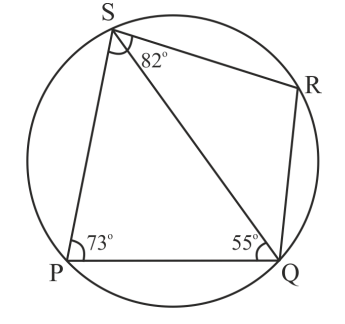
\includegraphics[scale=0.5]{figs/fig1.png}
    \caption{Problem figure}
    \label{fig:my_label}
\end{figure}

\end{center}
PQRS is a cyclic quadrilateral. Given \angle $QPS=73^o$, \angle $PQS=55^o$ and \angle $PSR=82^o$, calculate:\\
(i) \angle $QRS$\\
(ii) \angle $RQS$\\
(iii) \angle $PRQ$\\\\
\textbf {Solution: }\\\\
(i) We know that, In a Cyclic quadrilateral, sum of a pair of opposite angles results in $180^o$.
Hence,
\begin{center}
   $\angle QPS + \angle QRS = 180^o$
\end{center}
\begin{center}
$\rightarrow 73^o + \angle QRS = 180^o$
\end{center}
\begin{equation}
    \Rightarrow \angle QRS = 107^o
\end{equation}
(ii) Again, from the fact that sum of a pair of opposite angles is $180^o$,
\begin{center}
    $\angle PSR + \angle PQR = 180^o$
\end{center}
\begin{center}
    $\rightarrow 82^o + \angle PQS + \angle RQS = 180^o $
\end{center}
\begin{center}
    $\rightarrow 82^o + 55^o + \angle RQS = 180^o$
\end{center}
\begin{equation}
    \Rightarrow \angle RQS = 43^O
\end{equation}
(iii) We know that in a circle, a chord always subtends equal angles at all the points on a particular arc. Consider the chord "PQ",
\begin{equation}
    \rightarrow \angle PSQ = \angle PRQ
\end{equation}
We know that the sum of angles in a triangle equals to $180^o$, Consider the triangle $\triangle PQS$,
\begin{center}
    $\rightarrow \angle PSQ + \angle SPQ + \angle PQS = 180^o$ 
\end{center}
\begin{center}
    $\rightarrow \angle PSQ + 73^o + 55^o = 180^o $
\end{center}
\begin{center}
    $\rightarrow \angle PSQ = 52^o$
\end{center}
Substituting this result in the equation (3),
\begin{equation}
    \Rightarrow \angle PRQ = 52^o
\end{equation}\\\\
\newpage
Before construction of the figure, let us try and find out some of the required angles in plotting it.\\

In the figure, label the centre of the circle as "C", and join the points "P", "Q", "R", "S" to it. Make a diagram such that the point "P" is at the rightmost point of the figure. \\
\begin{figure}[ht]
    \centering
    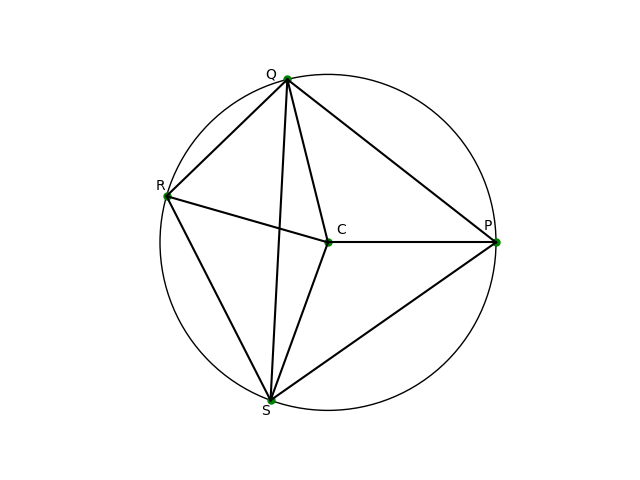
\includegraphics[scale = 0.5]{figs/pre_cnstrct_fig1.png}
    \end{figure}\\
Let,\\\\
$\angle CPQ = x$, $\angle CSP = y$, $\angle CRS = z$, $\angle CQR = \alpha, \angle CSQ = \theta .$\\\\
As the triangles, $\triangle CPS$, $\triangle CSR$, $\triangle CRQ$, $\triangle CQP$ and $\triangle CQS$ are isoceless,\\\\
$\angle CPQ = \angle CQP = x$\\
$\angle CSP = \angle CPS = y$\\
$\angle CRS = \angle CSR = z$\\
$\angle CQR = \angle CRQ = \alpha$\\
$\angle CQS = \angle CSQ = \theta$\\\\
We hope to find each of the angles that the chords, "PQ", "QR", "RS", "SP" make at the center, i.e., the angles, $"\angle PCQ", "\angle PCS", "\angle SCR", "\angle RCQ"$.\\\\
From the given information and the results we previously obtained, we can see the following equations being true.

\begin{equation}
    x + y = 73^o
\end{equation}
\begin{equation}
    y + \theta = 52^o
\end{equation}
\begin{equation}
    x + \theta = 55^o
\end{equation}
\begin{equation}
    y + z = 82^o
\end{equation}
\begin{equation}
    z + \alpha = 107^o
\end{equation}
\begin{equation}
    \alpha + x = 98^o
\end{equation}

On solving the above equations, we can obtain the values of the variables as, $x = 38^o, y = 35^o, z = 47^o, \alpha = 60^o .$\\\\
From these values of the variables, we can see that,\\\\
$\angle PCQ = 180^o - 2x = 104^o$\\
$\angle PCS = 180^o - 2y = 110^o$\\
$\angle RCQ = 180^O - 2\alpha = 60^o$\\\\
As $\angle PCR = \angle PCQ +\angle QCR$,\\ $\angle PCR = 104^o + 60^o = 164^o$.\\

\textbf{\underline{Construction of the given figure}: }\\\\
1) Draw a circle of radius "4" units with the centre "C".(The radius mentioned here is just for scale). Now as a reference point, label the point "P" at the rightmost end of the circle and join them.
\begin{figure}[ht]
    \centering
    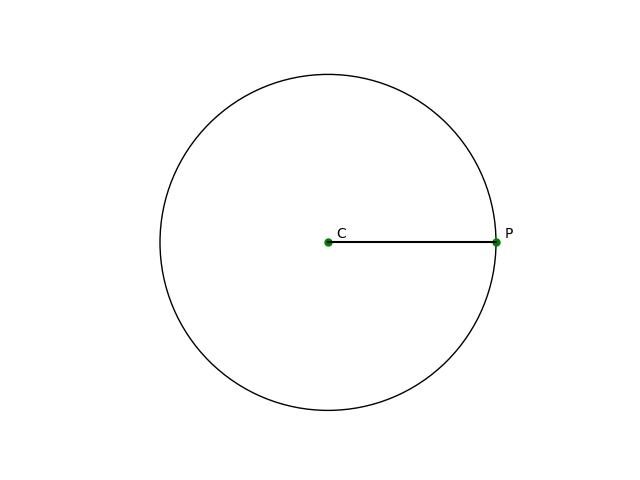
\includegraphics[scale = 0.5]{figs/cnstrct_fig1.png}
\end{figure}\\
\newpage
2) As we now know the angles made by the line segments "CQ", "CR", "CS" with the drawn line segment "CP", plot them using a protractor.
\begin{figure}[ht]
    \centering
    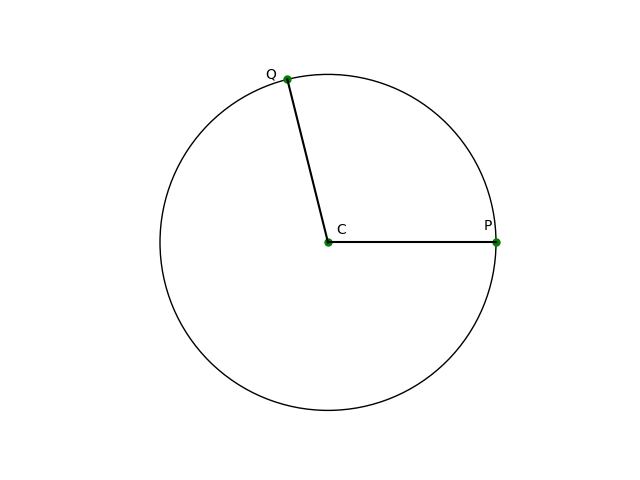
\includegraphics[scale = 0.5]{figs/cnstrct_fig2.png}
\end{figure}\\
3) Now join the vertices on the perimeter of the circle to produce the required cyclic quadrilateral.
\begin{figure}[ht]
    \centering
    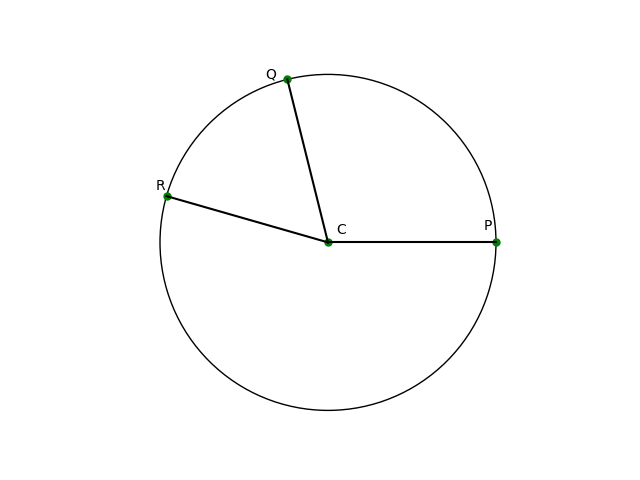
\includegraphics[scale = 0.5]{figs/cnstrct_fig3.png}
\end{figure}\\

In this manner, one can construct the given cyclic quadrilateral.

\end{document}
